\documentclass[english]{ntnuthesis}

% Make index:
\usepackage{makeidx}

\usepackage{hyperref}
\usepackage{listings}
\usepackage[T1]{fontenc}
\usepackage[landscape,a4paper]{geometry}
\usepackage{booktabs} 
\usepackage{colortbl} 
\usepackage{xcolor} 
\usepackage{xfrac}
%\usepackage[latin1]{inputenc}
\usepackage[english]{babel}
\usepackage{appendix}
\usepackage{textcomp}
\usepackage[binary,squaren]{SIunits}
\usepackage{amsmath, amsfonts, amssymb}
\usepackage{graphicx, subfigure, wrapfig}
\usepackage{listings}
\usepackage{multirow}
\usepackage[subfigure]{tocloft}
\usepackage{acronym}
\usepackage{lmodern}
\usepackage{pdfpages}
\usepackage{subcaption}
\usepackage{makecell}
\usepackage{url}

% MATLAB: load package with ``framed'' and ``numbered'' option.
\usepackage[framed,numbered]{mcode}

\usepackage{algorithm,algorithmicx,algpseudocode}
\algnewcommand\algorithmicto{\textbf{to}}

% Do not use bullets in un-numbered lists:
\renewcommand{\labelitemi}{\normalfont\textendash}
\renewcommand{\labelitemii}{\normalfont\textperiodcentered}

% Do not use dot after speaches in numbered lists:
\usepackage[pointlessenum]{paralist}

% Accept comma as fraction separator in math expressions
% (This package is much smarter than the icomma-package.)
\usepackage{ncccomma}

% Macro for microseconds
\newcommand{\us}{\,$\mu$s}

% Define AVR32 assembly
\lstdefinelanguage{avr32asm}{
morekeywords={lddpc,mov,st.w,cp.w,cp.b,bfextu,breq,
brne,rete,sub,rjmp,lsl,lsr,com,st.w,ld.w,csrf,mtsr,
rcall,reteq,br,ret,.int,.include,.globl},
  sensitive=false,
morecomment=[l]{//},
morecomment=[s]{/*}{*/},
alsodigit={.},
}

\lstloadlanguages{c, c++, avr32asm, vhdl}

% Used with the make index package
\makeindex

\begin{document}
\hyphenpenalty=8000
\exhyphenpenalty=8000
% Write how to divide long words:
\hyphenation{temp-tation}

\frontmatter

\title{Dual RISC-V cores for glitch protection}

\author{ Jarl Magnus Sæbø }
\degreetype{Design of Digital and Embedded Systems}

\maketitle
%\includepdf{titlepage}
%\includepdf{problemdes}
% Insert page number
\setcounter{page}{5}
\chapter{Abstract}

This project aims at using the CV32E40S RISC-V CPU in a dual-core lockstep mechanism as a way of doing glitch protection. The purpose of this research is to determine whether this simple measure can replace pre-existing and much more complex security features. By proving the effectiveness of this new hardware architecture, it paves the way for developers to simplify their designs and speed up the development of future CPUs. In addition, this project aims at broadening the public knowledge about secure CPU design, as this topic is largely kept a secret by the major players in the industry. 

To address this, all research was done on an open-source RISC-V core. This core contains a lot of complex security features, which were found to add a somewhat significant amount of resource usage. By simply disabling one of the many security features the overall performance of the system could be increased by 5\%. To compare the quality of the dual-core setup with the existing setup, they were both subjected to different types of simulated glitch attacks while running a simple test program. From these tests we found that the dual-core setup was just as capable of detecting errors, and even surpassed the existing setup in some cases. This means that it is a simple and viable alternative for researchers aiming to secure their hardware against glitch attacks. 

To advance this research, the next phase involves fabricating an actual chip based on the proposed architecture and assessing its resilience against various real-world glitch attacks. Specific focus will be given to electromagnetic fault injection, voltage manipulation, and clock glitching techniques, which pose substantial threats to modern computing systems. This comprehensive evaluation will provide important insights into the practical viability of the dual-core lock-step mechanism as a security solution for RISC-V cores.

\chapter{Preface}
I would like to thank....


\cleardoublepage

% Remove parskip for toc
\setlength{\parskip}{0ex plus 0.5ex minus 0.2ex}
\thispagestyle{fancyplain}
\setcounter{tocdepth}{3}
\tableofcontents


\cleardoublepage
\listoftables
\cleardoublepage
\listoffigures
\cleardoublepage
\renewcommand{\lstlistlistingname}{Source code}
\lstlistoflistings

\chapter{List of abbreviations}
\begin{acronym}
\acro{PC}{Program Counter}
\acro{PCH}{Program Counter Hardening}
\acro{CSR}{Control and Status Register}
\acro{IF}{Instruction Fetch}
\acro{ID}{Instruction Decode}
\acro{EX}{Execute}
\acro{WB}{Write Back}
\acro{LSU}{Load Store Unit}
\acro{DCL}{Dual-Core Lockstep}
\acro{CPU}{Central Processing Unit}
\acro{RISC}{Reduced Instruction Set Computer}
\acro{ISA}{Instruction Set Architecture}
\acro{ISE}{Instruction Set Extension}
\acro{ECC}{Error Correcting Code}
\acro{EMFI}{Electromagnetic Fault Injection}
\acro{SoC}{System on Chip}
\acro{PPA}{Power Performance Area}
\acro{RTL}{Register Transfer Level}
\acro{ASM}{Assembly}
\acro{TEE}{Trusted Execution Environment}
\acro{PMP}{Physical Memory Protection}
\acro{OBI}{Open Bus Interface}


%\acro{}{}
\end{acronym}

\cleardoublepage

\mainmatter

\chapter{Introduction}
\label{intro} 

Modern integrated systems and other programmable electronics often have safety-measures built in to avoid unintended behaviour, whether it be accidental or from an external source. These safety measures typically only address software or firmware issues, leaving systems unprotected against hardware-induced faults, known as glitch attacks. These attacks are able to bypass robust software and firmware security measures given the right method of attack. Interestingly, despite the importance of glitch protection, it only started gaining attention after practical glitch attacks first made their appearance in 2002 through an optical fault attack\cite{trouchkine2019fault}. 

In the world of computer architecture, many aspects remain closely guarded secrets, including preventive measures against glitch attacks. This secrecy often makes these preventative measures inaccessible to the public. Over recent years there has been a large shift away from this secrecy as more and more researchers and companies use the \textit{RISC-V} instruction set architecture (ISA)\cite{riscv_manual}. This architecture is open source, allowing anyone with the right knowledge and motivation to create their own central processing unit (CPU). One group of people doing this is the \textit{OpenHW Group} who have developed several publicly available RISC-V CPUs over recent years. One of these is the \textit{CV32E40S}, which is a core mainly focused on safeguarding against glitch- and side-channel attacks\cite{cv32e40s_manual}.

While the \textit{CV32E40S} has a proven to be able to detect glitch attacks, it comes at a cost in performance. Often the methods used to protect against attacks are complex and increase the execution time and power needed for the CPU to perform its given tasks. This project investigates the possibility of replacing some of the security features of the \textit{CV32E40S} in favour of running two CPUs in a \textit{Dual-Core Lockstep} (DCL) mechanism instead to increase throughput and simplicity. Henceforth the core using the DCL mechanism is reffered to as the \textit{CV32E40DC}. 

\section{Sustainability}
\label{sec:sustainability}

Out of the 17 sustainability goals of the United Nations\cite{un}, at least two can be considered highly relevant for this project. 

\begin{itemize}
    \item \textbf{Goal 9:} Build resilient infrastructure, promote sustainable industrialization and foster innovation.
    \item \textbf{Goal 17:} Revitalize the global partnership for sustainable development.
\end{itemize}

The goal of this project is to investigate a new way of possibly making components more resilient against attacks and exploits. This fits into \textit{goal 9}. In addition, this project works to increase the knowledge around an open source project. Being open source means anyone in the world can access all parts of the code. This is relevant for promoting \textit{goal 17} of revitalizing global partnership for sustainable development. 

\section{The use of AI}
\label{sec:AI}

The AI chat bot ChatGPT made by \textit{Open AI}\cite{chat} was used as an academic tool when working on this project. Its main use was to offer possible ways to restructure parts of the text that could be difficult to understand or where the point did not come across clearly. For example, I had the following text where the word "them" could be ambiguous: 

\begin{lstlisting}
Restructure this sentence so its more clear what "them" is: 
In the world of computer architecture, many aspects remain closely guarded
secrets. This secrecy extends to preventive measures against such 
attacks, making them often inaccessible to the public.
\end{lstlisting}



In addition it was used to generate code that would otherwise be tedious to write. This includes for example SystemVerilog code where two modules with large interfaces are connected. 
%\chapter{State of the art}
\label{chap2}

% Today micro-controllers and other embedded electronics are in almost everything we use. Because of this, ensuring the secure operation of these devices is critical. While much attention is directed towards software and firmware security, hardware security often goes overlooked. Particularly, hardware fault-injection (glitching) has repeatedly demonstrated its capability to bypass conventional security measures. Examples include bypassing cryptographic signature validation of firmware binaries \cite{hole_in_soc}, re-enabling hardware debug functionality on production/fused processors\cite{reenable_debug} and bypassing input validation of data that crosses trust boundaries between privilege levels\cite{qualcom}. To stop these glitch attacks, a number of countermeasures can be introduced. This project looks at the ones implemented by the OpenHW Group for their 'CV32E40S' RISC-V core\cite{cv32e40s_manual}, and how these security measures can be avoided entirely by instead running a dual-core RISC-V setup with lockstep. 
% After the discovery of the first glitch attack in 2002, many other examples have followed. These include bypassing cryptographic signature validation of firmware binaries \cite{hole_in_soc}. This was done using voltage glitching to bypass the verification of a firmware images signature. re-enabling hardware debug functionality on production/fused processors\cite{reenable_debug} and bypassing input validation of data that crosses trust boundaries between privilege levels\cite{qualcom}.

The RISC-V architecture has over recent years gained a lot of traction in both academia and industry due to its modular design and adaptability\cite{source2}. However, due to the nature of open source resources, RISC-V systems are often more susceptible to glitch attacks as hackers can research the ISA in depth to find errors. This was done in 2021 by two researchers\cite{isa_exploit}. What they found was that in the ISA there was never specified a base address for the \textit{Machine Trap Vector} (MTVEC) before booting up a RISC-V core. As the MTVEC is resposnsible for handling exceptions, this lead to an exploitable issue: If an attacker were to induce some exception during boot, it would be handled by the MTVEC. However, as the MTVEC had no base address (0x00000000) it would raise another exception. This then leads to an infinite exception loop which can be exploited. In addition to this vulnerability due to the availability of sensitive information, the actual chips made with the RISC-V architecture will still be susceptible to more common attacks like electromagnetic fault injection (EMFI) or voltage- and clock-glitching. 

% Often the security measures that are implemented aim at stopping one specific form of attack. Take for instance the example code shown in \autoref{fig:glitchable_code}. This code represents a secure boot process where first an image is fetched. The result code of the fetch operation is then checked to see whether the correct image was fetched, or if an error occurred. In the case of the latter, the program is stuck in in an infinite loop and if not the boot process can continue. From the figure one can observe that there exists a number of weak points that can be exploited. Because of this hardware designers implement things like \textit{Program Counter Hardening} (PCH) to check for instruction skips by comparing current and expected PC values, and \textit{Error Correcting Code} (ECC) to validate data integrity in registers. However, while these features would stop an attacker in this example, what if the attacker finds a way to boot with the wrong PC and start at the 'do\_boot' instruction? In this case we would need to develop a new form of protection with a greater fault detection coverage. Such a solution is discussed in this project in the form of a dual-core lockstep mechanism. 

% \begin{figure}[h!]
%     \centering
%     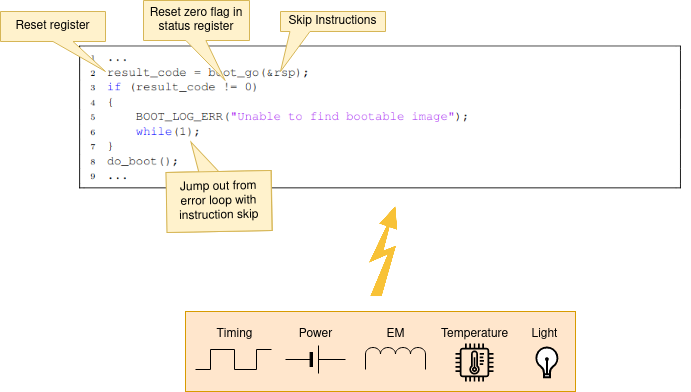
\includegraphics[width=0.75\textwidth]{docs/images/glitch_attack_whole_system.png}
%     \caption{Example of code that can be glitched with common attacks. \textit{Figure inspired by one found in “Fault Attacks on Secure Embedded Software:
% Threats, Design and Evaluation”, Bilgiday Yuce, Patrick Schaumont,
% Marc Witteman}}
%     \label{fig:glitchable_code}
% \end{figure}


 
%4. Scope of the Problem:

%System Vulnerabilities: An in-depth understanding of where and how glitches typically affect RISC-V cores is crucial. This entails both functional and performance impacts.
%Dual Core Strategy: Introducing a dual-core setup offers potential glitch protection via redundancy. However, the feasibility, overheads, synchronization mechanisms, and actual effectiveness of such a strategy need thorough examination.
%Protection Mechanisms: Beyond the mere introduction of dual cores, the strategies for detection of a glitch, switch-over mechanisms, and potential recovery strategies need to be explored.
%5. Objectives:

%The primary objectives for this project include:

%Conducting a vulnerability analysis of single-core RISC-V systems concerning glitches.
%Designing a dual-core RISC-V system prototype aiming for glitch protection.
%Evaluating the effectiveness of the dual-core setup in real-world scenarios and benchmark tests.
%Proposing additional countermeasures or strategies, if needed, to enhance glitch protection further.
%6. Significance:
%By addressing the problem defined, this project aims not only to enhance the reliability of RISC-V based systems but also to contribute to the broader realm of glitch protection in electronics. With the ever-increasing adoption of RISC-V in various applications, ensuring its robustness against glitches will be paramount for many industries.


\chapter{Background \& State of the art}
\label{chap3}

This chapter describes what glitch attacks are, why developers need to protect their devices from them and the current limitations related to this. The \textit{CV32E40S} RISC-V core by the OpenHW group is also introduced, and the potential benefits of replacing some of its security features are investigated. 

\section{What are glitch attacks?}
\label{sec:glitch_attacks}

Glitch attacks, also known as hardware fault injection, are a sophisticated form of hacking aimed at exploiting vulnerabilities in hardware systems. The primary objective is to disrupt normal execution to bypass security features in order to gain access to sensitive data, bypass authentication protocols or undermine cryptographic operations. 

Glitch attacks can be divided into two main categories: invasive (e.g., decapsulating the chip\cite{intro_to_hw_hacking}) and non-invasive attacks (e.g., electromagnetic fault injection (EMFI), voltage- and clock-glitching). Often times software and firmware security measures can only protect against non-invasive glitches, as protecting from invasive glitches often require hardware modifications\cite{glitchresistor}. Due to the nature of invasive attacks, it is beyond the scope of this project to defend against them. This is because these often aim at tampering with Read-Only Memory (ROM) or Boot-loaders on Printed Circuit Boards (PCBs), and are not effective against more complex systems like a Central Processing Unit (CPU) or a System on Chip (SoC). Therefore, protecting against these attacks is the responsibility of other components than the core.

\subsection{Non-invasine glitch attacks}
\label{sec:non_invasive}

Non-invasive glitches can be performed as long as an attacker has access to a device. However, there is quite a lot of procedural vulnerability discovery that has to be done before an attack can be performed\cite{arm_presentation_2}. In the case of Electromagnetic Fault Injection (EMFI) the chip has to be repeatedly exposed to electromagnetic interference during execution, to then determine which areas are most vulnerable to attacks\cite{emfi_injection}. An example of such probing having been performed on the BCM2837 SoC can be seen in \autoref{fig:emfi_map}\cite{emfi_injection}. 

Voltage- or clock-glitching can be performed as long as there is some way to access these signals externally. Voltage-glitching often requires the removal of power filtering capacitors to gain more fine-grained control over a processor's voltage input. However, both of these methods require very precise timing by an attacker. This is why specialized tools such as the \textit{ChipWhisperer}\cite{chipWhisperer} were made, as they allow for extremely accurate fault-injection. These days it is also possible to perform effective glitch attacks with simple components in conjunction with a cheap Field Programmable Gate Array (FPGA) which outputs precise triggers as shown in\cite{hole_in_soc}. 

\begin{figure}[h!]
    \centering
    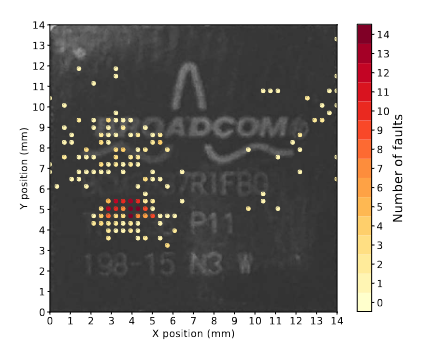
\includegraphics[scale=0.5]{docs/images/emfi_error_map.png}
    \caption{EMFI BCM2837 sensitivity map (dot size is not corralated with probe size.)\cite{emfi_injection}.}
    \label{fig:emfi_map}
\end{figure}

Voltage-glitching is performed by momentarily dropping the supply voltage during execution of critical operations. Clock-glitching is performed by altering clock timing to violate setup and hold time requirements of the hardware\cite{intro_to_FI}. The results of glitches cannot always be predicted, however they mainly result in skipped or repeated CPU instructions, incorrect evaluation of CPU instructions or corrupt reads from memory devices\cite{intro_to_FI}. In general these faults can occur at any stage in the execution pipeline. A typical application for these types of glitches is to skip some sort of signature verification in a bootloader or other security module. Take for instance the example code shown in \autoref{fig:glitchable_code}. This example shows an example of secure boot code. This is often a target for attacks as the execution time is deterministic, and given physical access to the device an attacker can try as many times as they want to bypass the authentication process \cite{arm_presentation}. 

In the code in \autoref{fig:glitchable_code} a boot image is first fetched. The result code of this operation is then checked to see whether the correct image was fetched, or if an error occurred. In the case of an error, the program is stuck in in an infinite loop. If the correct image was fetched the boot process can continue. From the figure we see that there exists a number of weak points that can be exploited using common forms of attacks. For example voltage- or clock-glitching could be used to bypass the 'boot\_go' function or jump out of the infinite while loop. EMFI and laser pulse attacks often offer a higher degree of spatial and temporal precision. This allows attacks to more effectively target specific pipeline stages, and could therefore be used to disrupt the conditional check or status registers\cite{intro_to_FI}. 

\begin{figure}[h!]
    \centering
    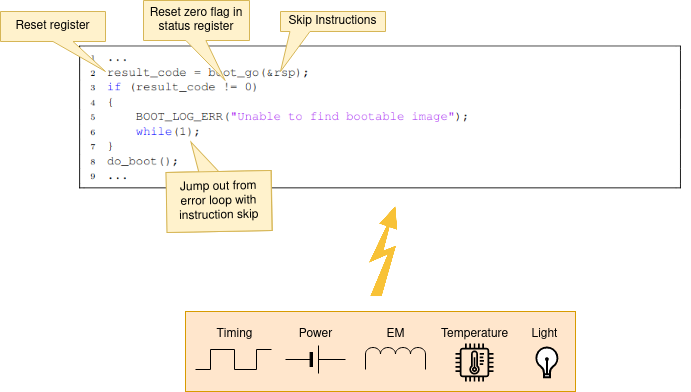
\includegraphics[width=0.75\textwidth]{docs/images/glitch_attack_whole_system.png}
    \caption{Example of code that can be glitched with common attacks. Figure inspired by one found in \cite{arm_presentation}.}
    \label{fig:glitchable_code}
\end{figure}

Because of this hardware designers often implement security features aimed at protecting against specific forms of attacks. This includes thins like \textit{Program Counter Hardening} (PCH) to check for instruction skips by comparing current and expected PC values, and \textit{Error Correcting Code} (ECC) to validate data integrity in registers\cite{cv32e40s_manual}. However, while these features would stop an attacker in this example, what if the attacker finds a way to boot with the wrong PC and start the program at the 'do\_boot' function? In this case we would need to develop a new form of protection with a greater fault detection coverage. Such a solution is investigated in this project in the form of a DCL mechanism in the \textit{CV32E40DC}. 

% Glitch attacks have over recent years become a more common and greater threat. Due to the nature of how these attacks are carried out, they are often a very affordable way to exploit hardware. Attackers have easy access to open source resources like the the 'ChipWhisperer Lite' which allows for easy access to hardware glitching tools as well as side channel analysis\cite{chipWhisperer}. In addition to this, FPGAs can be used to inject precisely timed faults as long as an attacker has access to the supply voltage or clock on a chip\cite{hole_in_soc}. 

\section{The need for glitch protection}
\label{sec:need}

Within the world of CPU design the two biggest architectures are ARM and x86 (produced by Intel and AMD). Most of the devices we use every day has one of these types of chips inside them, and because of this they also implement several security features to prevent glitch attacks. For ARM processors this includes, among other things, the \textit{TrustZone} which provides hardware-enforced isolation between trusted and non-trusted software, as well as built in physical attack protection\cite{arm}. The 12th generation x86 processors produced by Intel have a Tunable Replica Circuit (TRC), which uses hardware-based sensors to explicitly detect circuit-based timing failures that occur as the result of an attack\cite{intel}.  

Unfortunately, for many years the details of CPU design have been hidden from the public due to the strict secrecy producers have around their products\cite{riscv_wiki}. While this limits what the public can know, it also means that a potential hacker would have a much harder time finding exploits in the architecture. However, due to the nature of open source projects, this is a larger vulnerability for products based on the RISC-V instruction set architecture (ISA). An example of direct exploitation of the ISA was shown during the 'DEFCON' conference in 2019\cite{isa_exploit}. Here it was demonstrated that triggering an exception during boot of a RISC-V chip would lead to an 'exception loop'. This was because the Machine Trap Vector (MTVEC) had no base address before boot (e.g., it was set to 0x0). Pointing to this address is permitted in the ISA, and doing so will trigger an exception. This means that triggering an exception before boot leads to the exception handler pointing to an illegal address, which again triggers an exception and this continues forever. Handling of exceptions happens first at the highest privilege mode (Machine mode), which means that the chip is also stuck in this mode. The RISC-V architecture is designed with some key security features in mind. One of these are the previously mentioned privilege levels. These are in descending order: machine (M-mode), hypervisor (H-mode), supervisor (S-mode) and user mode (U-mode). A higher privilege mode can access all the functions used in a lower privilege mode\cite{source2}.

Other key security features in the RISC-V architecture are the physical memory protection (PMP), and the trusted execution environment (TEE). The PMP ensures that no access is given to protected parts of the memory region. The TEE is a secure and isolated area within a computer system that provides a higher level of security for processing sensitive information. One of the main objectives of the PMP and the privilege levels is to provide a TEE that isolates secure and insecure applications. It is critical for software and firmware developers that these features work. However, as shown in \cite{source2} the integrity of TEEs can be bypassed using clock-glitching. 

%\section{Previous Approaches to glitch protection}
\section{CV32E40S by the OpenHW group}
\label{sec:cv32}

The previously mentioned security measures of the RISC-V ISA do a decent job at protecting against glitch attacks, but as mentioned they can be bypassed. Therefore there is a need for more specialized security features. Because of this the \textit{OpenHW} group developed the \textit{CV32E40S}. This is a 4-stage in-order 32-bit RISC-V processor core with the main intention of ensuring secure operation\cite{cv32e40s_manual}. This core has the same privilege modes and PMP as described to ensure a TEE. There are however implemented extra security features through an Instruction Set Extension (ISE), \textit{Xsecure}. The CV32E40S started out as a fork of the CV32E40P which is another RISC-V processor made by the OpenHW group. The top-level block diagram of the CV32E40S core is shown in \autoref{fig:cv32e40s_block}. From the figure one can see that the architecture of this core is much like any other RISC-V core, with an Instruction Decode, Instruction Fetch, Execute and Write Back stage. 

%The extra security features of this core are a PCH module in the IF stage (not shown in figure), ECC in the register file in the ID and CSR Hardening in the EX stage. 

\begin{figure}[h!]
    \centering
    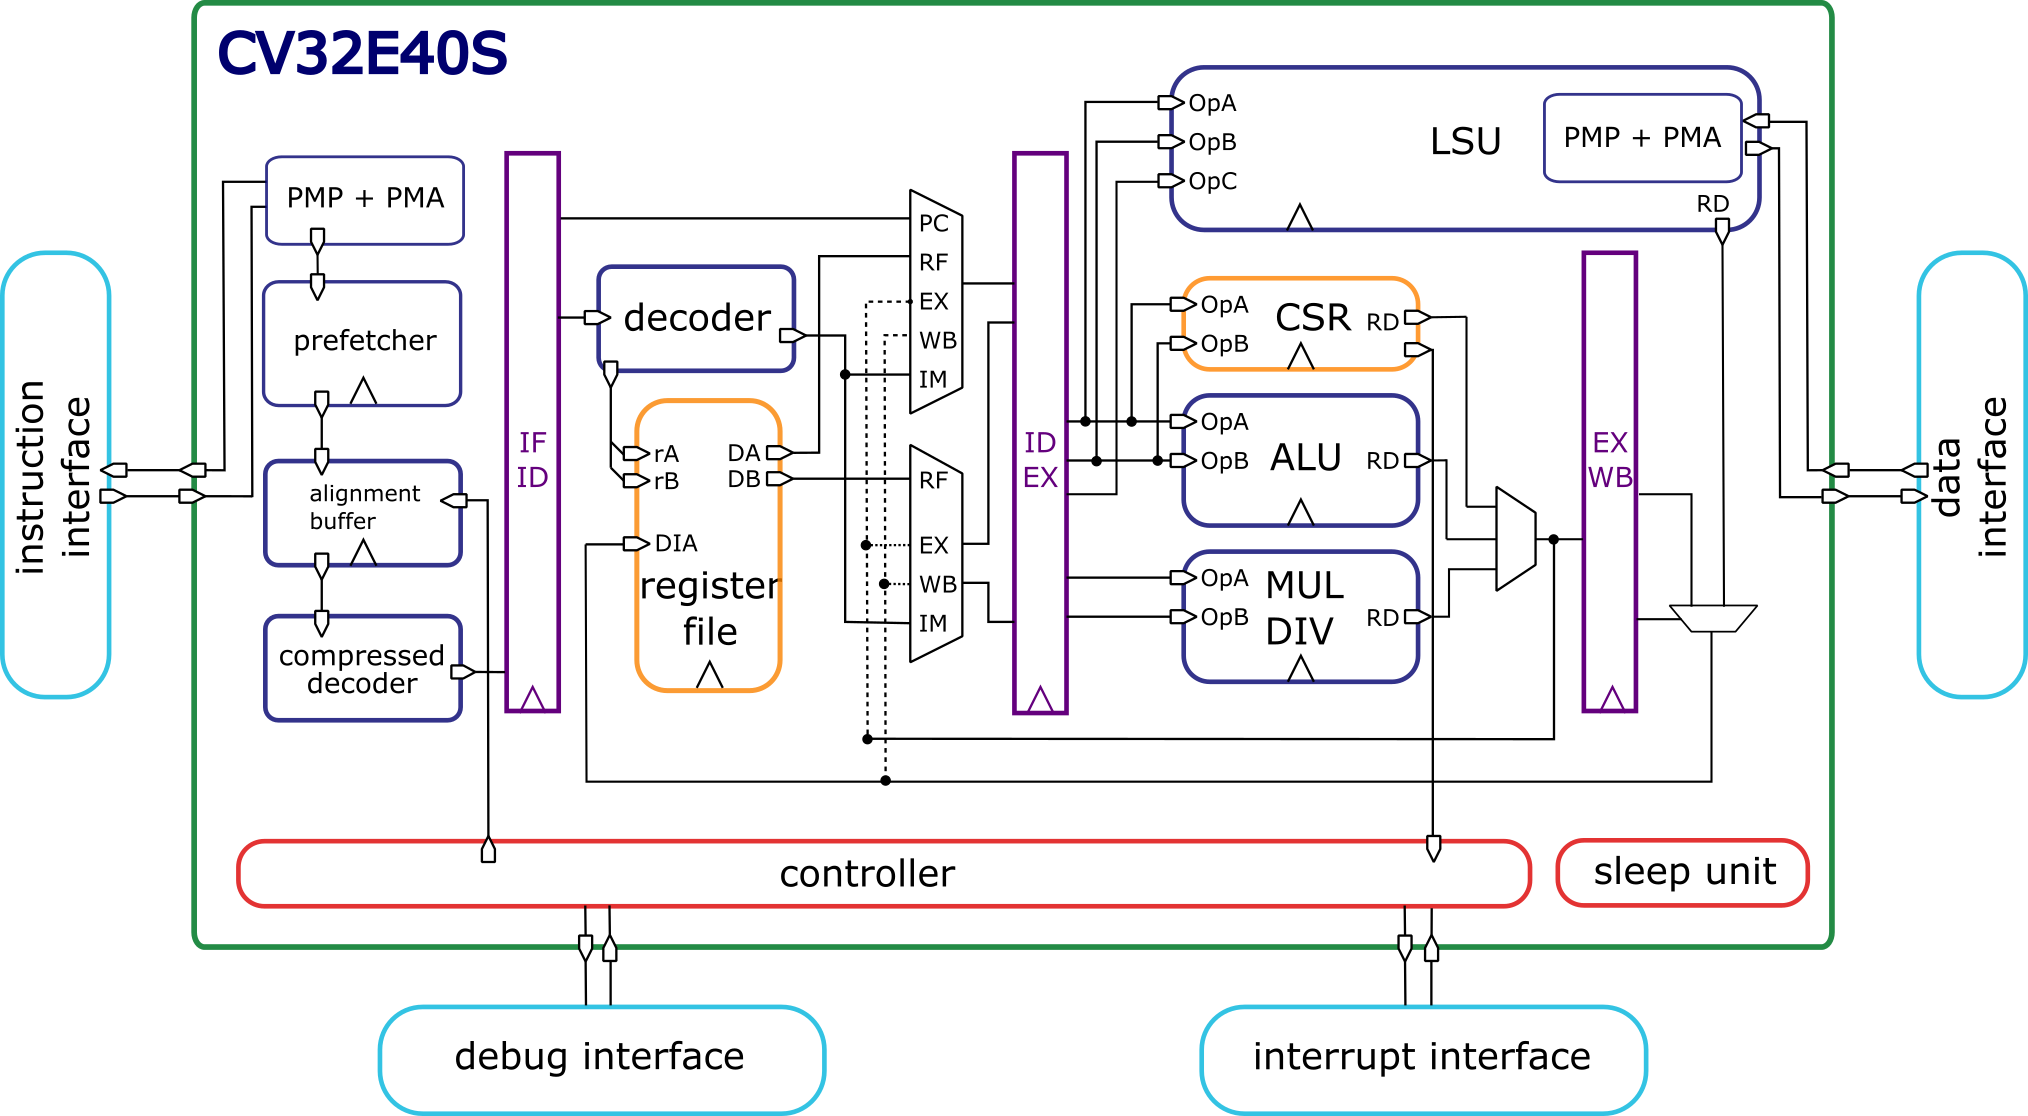
\includegraphics[width=0.8\textwidth]{docs/images/CV32E40S_Block_Diagram.png}
    \caption{CV32E40S top-level block diagram\cite{cv32e40s_manual}.}
    \label{fig:cv32e40s_block}
\end{figure}

\subsection{Xsecure Extension}
\label{sec:xsecure}

\textit{Xsecure} is an ISE that adds extra security features to the CV32E40S core. These are aimed at protecting against side-channel attacks as well as glitch attacks. Protection against side channel attacks is done using \textit{data independent timing (DIT)}, \textit{dummy instruction insertion} and \textit{random instructions}\cite{cv32e40s_manual}. These features will increase execution time for the core. However, they cannot easily be replaced with the use of the DCL mechanism. This is because preventing side-channel attacks is less about redundancy and more about making the power usage or execution time of a processor unpredictable. 

The extension also adds specific features to prevent glitch attacks. Three such features that will be discussed further in this report are: \textit{Register file Error Correcting Code (ECC)}, \textit{Program Counter Hardening (PCH)} and \textit{Control and Status Register Hardening (CSRH)}. The main goal of this project is to investigate whether these can be replaced with a DCL mechanism. 

In order to gain some background knowledge about the impact these features have on the Power, Performance and Area (PPA) of the core we did some preliminary tests. These consisted of running the sanity check program in \autoref{lst:sample_code} to see the difference in execution time. In addition to this, both cores were synthesized to compare their area and power usage. Specifically removing only the ECC, PCH and CSRH features without also affecting the core as a whole is complicated. Because of this, the tests are only run with the PCH feature disabled. In addition the tests are run with and without DIT, as this feature adds a lot of 'artificial' execution time. This way we get some insight into the impact the PCH feature has on its own, and during normal execution when everything is enabled. 

\autoref{tab:synth_ppa} shows the area and power usage of both cores after synthesis. We can see that area decreases by $2.2\%$ and power usage by $1.5\%$ when PCH is removed. Both cores ran the simulated program, and \autoref{tab:simulation_cc} shows that running the program with PCH enabled requires 9 extra clock cycles with DIT enabled. When DIT is disabled the number of clock cyles is reduced by 843. This represents a $0.05\%$ and $4.86\%$ decrease respectively. The documentation for the core states that \textit{jumps} as well as \textit{branches} that are not taken will require one extra clock cycle due to PCH. All branches are taken when DIT is enabled\footnote{branches that would not normally be taken are immediately followed up by killing of the fetch and decode stages}, which explains why the impact of PCH is so small with this feature on\cite{cv32e40s_manual}. As explained earlier a DCL mechanism will not be able to replace the side-channel attack prevention. Because of this the potential gain from removing the PCH feature is in this case limited to $0.05\%$. 

From the results shown in \autoref{tab:synth_ppa} and \autoref{tab:simulation_cc} one can argue that PPA alone is not a valid reason to replace the glitch protection features of \textit{Xsecure}. However, because the extension adds features aimed at only covering specific parts of the core, an attacker can bypass these by targeting an uncovered area. These shortcomings can, at the cost of area and power consumption, be solved with the use of a DCL mechanism. The main advantage of this will then be fault detection coverage as well as robustness. If all inputs and outputs of two cores are continuously compared, a fault in any part of either of them will be detectable.  

\begin{table}[h]
\centering
\caption{Synthesized resource usage with and without \textit{PC-Hardening}.}
\label{tab:synth_ppa}
\begin{tabular}{ccc}
\toprule 
& With PC-Hardening & Without PC-Hardening \\
\midrule
\rowcolor{black!20} \textbf{area[$pm^2$]} & 63121.093 & 61757.916[$-2.16\%$] \\
\textbf{power[$\mu W$]} & 113.007 & 110.450[$-2.26\%$] \\
\bottomrule
\end{tabular}
\end{table}

\begin{table}[h]
\centering
\caption{Number of clock cycles needed to simulate the program in \autoref{lst:sample_code} with and without \textit{PC-Hardening}.}
\label{tab:simulation_cc}
\begin{tabular}{c|cc}
\toprule 
Data Independent Timing & With PC-Hardening & Without PC-Hardening \\
\midrule
\rowcolor{black!20} enabled & 18424 & 18415[$-0.05\%$] \\
disabled & 17313 & 16470[$-4.86\%$] \\
\bottomrule
\end{tabular}
\end{table}

% \begin{figure}[h!]
%     \centering
%     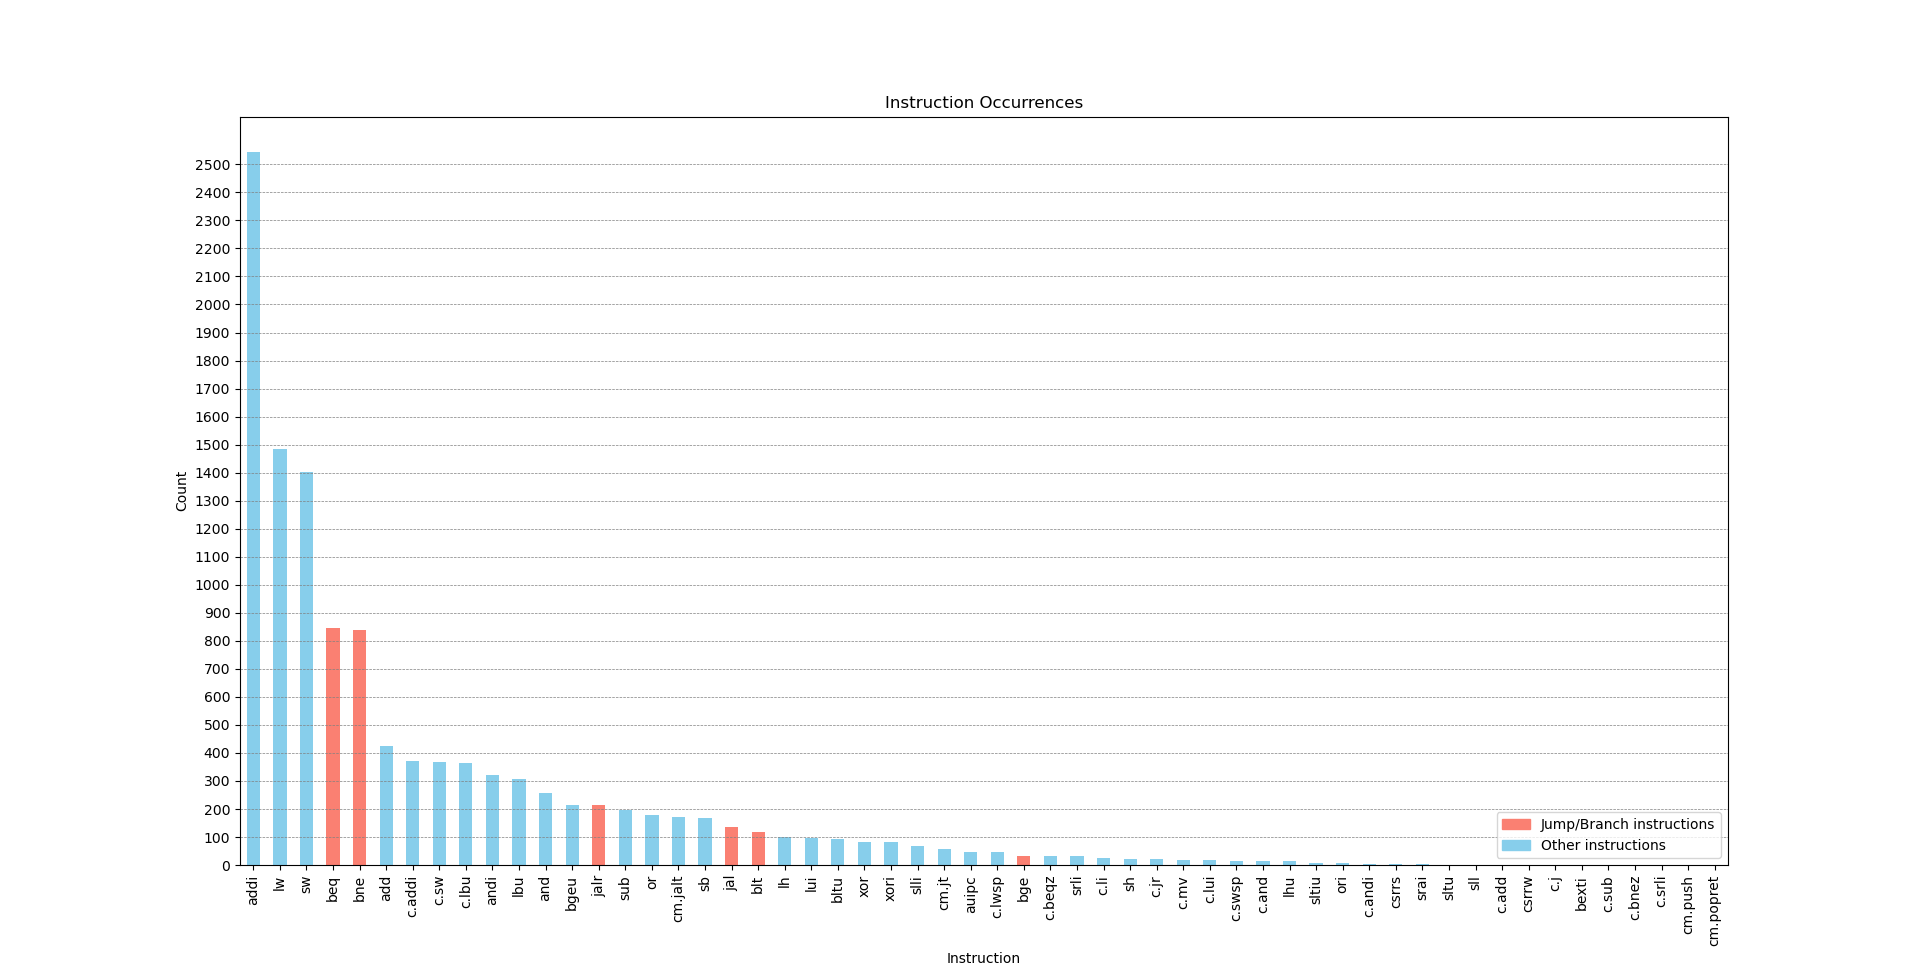
\includegraphics[width=\textwidth]{docs/images/instruction_occurances_all_legend.png}
%     \caption{All instructions in the generated assembly for the \textit{hello-world}\autoref{app:helloworldC} example, and the amount of calls for each instruction.}
%     \label{fig:instr_occ}
% \end{figure}


% \section{Limitations of glitch protection}
% \label{sec:limits}

% Despite greatly increasing the hardware security of devices, many glitch protection methods can have some common limitations. For instance the coverage of protection can often be incomplete. This means that designers often only focus on the most critical glitches, and can therefore sometimes overlook seemingly insignificant glitches that might break the system. For instance, a designer could implement a robust check to see whether the program counter has been modified during execution. However if an attacker glitches the program counter on boot, it could go undetected by the checker mechanism. 

% In general, glitch protection mechanisms will add to both the area and power consumption of a chip. Often the added area also comes from components that are logically redundant. In addition there will potentially be quite a lot of latency added. As previously described in \autoref{sec:xsecure}, the \textit{PC-hardening} module will add one extra cycle per jump or branch that is not taken. From \autoref{fig:instr_occ} it can be seen that even in a very simple program the potential for added latency is big. However, most of the potential performance gain that can be achieved from removing the \textit{Xsecure} features is mitigated by the side-channel safety features, which can not be removed. 

% From simulation and synthesis of both cores it is obvious that the argument for using a dual-core lockstep mechanism cannot be made solely on resource usage and performance gain alone. However, the main advantage will be the coverage and robustness gained. To test this claim, the regular and dual-core setups will both be subjected to several different glitch attacks that will take place in different parts of the pipeline. The quality of the solution will then be determined by how effective each setup is at responding to the attack. 

\section{Problem Definition}
\label{sec:problem_definition}

The \textit{OpenHW} group has developed the CV32E40S core which focuses on secure operation. A feature of this core is the ISE \textit{Xsecure} which introduces ways of mitigating side-channel attacks as well as glitch attacks. To stop glitch attacks the extension introduces features like ECC, CSRH and PCH that cover specific parts of the core. These can increase excution time, area and power usage of the core. This project investigates the possibility replacing these pre-existing security features in favour of using dual RISC-V cores in a lockstep mechanism. This will come at the cost of increased area and power usage. However, by continuously comparing all inputs and outputs of the two cores, we can achieve a greater level of fault coverage and robustness. 

To investigate the feasibility of the \textit{CV32E40DC} both cores will be synthesized and their PPA will be compared. In addition both will be tested against simulations of possible glitch attacks. The quality of our proposed architecture is determined by the ability to detect glitch attacks. The ability to fix the glitch or reset the core upon detection of a glitch is not investigated. This is because such things are handled by different parts of the system. PPA also plays a role in determining the quality of our solution. However, as the core is meant to be used in secure operations we allow an increase in power and area in favour of robustness. 

\chapter{Experimental}
\label{chap4}

\section{Methodology and theory}
\label{sec:method}

\subsection{How are the different layouts tested?}
\subsubsection{Synthesis tool - Which one is used?}
\subsubsection{How is fault injection done in sumlation?}
\subsection{How are results from fault injection compared between the different setups?}

\section{Limitations}
\label{sec:limit}

\section{Choices / Findings}
\label{sec:choice}
\chapter{Results and Analysis}
\label{chap5}

To perform the tests described in \autoref{tab:instr_skip_test} we follow the steps described in \autoref{subsec:sim_glitch}.

\section{PPA comparison}
\label{sec:synth_comparison}

Results of synthesis of both cores as well as number of cycles needed to complete the test program in \autoref{app:helloworldC} is shown in \autoref{tab:ppa_results}. The relative difference from the single core to dual-cores is shown in the table.

\begin{table}[h]
\centering
\caption{PPA results from simulation and synthesis of both setups.}
\label{tab:ppa_results}
\begin{tabular}{c|ccc}
\toprule 
Setup & Area[$pm^2$] & Power[$\mu W$] & Clock Cycles\\
\midrule
\rowcolor{black!20} CV32E40S & 63121.093 & 113.007 & 18424\\
CV32E40S Dual-Core & 65214.732[$+3.3\%$] & 144.482[$+27.9\%$] & 17446[$-5.3\%$] \\
\bottomrule
\end{tabular}
\end{table}

\section{Instruction Skipping}
\label{sec:instr_skip_result}

\subsection{CV32E40S}
\label{subsec:single_instr_skip}

\subsubsection{Skipping function call}

 From the log file, we can see that the \textit{c.jal} instruction is logged at 1752ns. To skip this instruction the program counter needs to be skipped in the \textit{IF} stage, which is 3 cycles before \textit{WB}. The system clock has a period of 3ns, meaning the glitch is injected at 1743ns. The \textit{c.jal} is located at the address: \textit{0x0000044c}. Forcing the program counter to the next address \textit{0x0000044e} for a duration of 3ns will simulate an instruction skip. The address of the next instruction is only 2 away because the \textit{jal} is a 16-bit compressed instruction.

Glitching of the core was done successfully. The waveforms from simulation are shown in \autoref{fig:instr_skip_single_wave}. From the figure one can see that the glitch is detected immediately. 

\begin{figure}[h!]
    \centering
    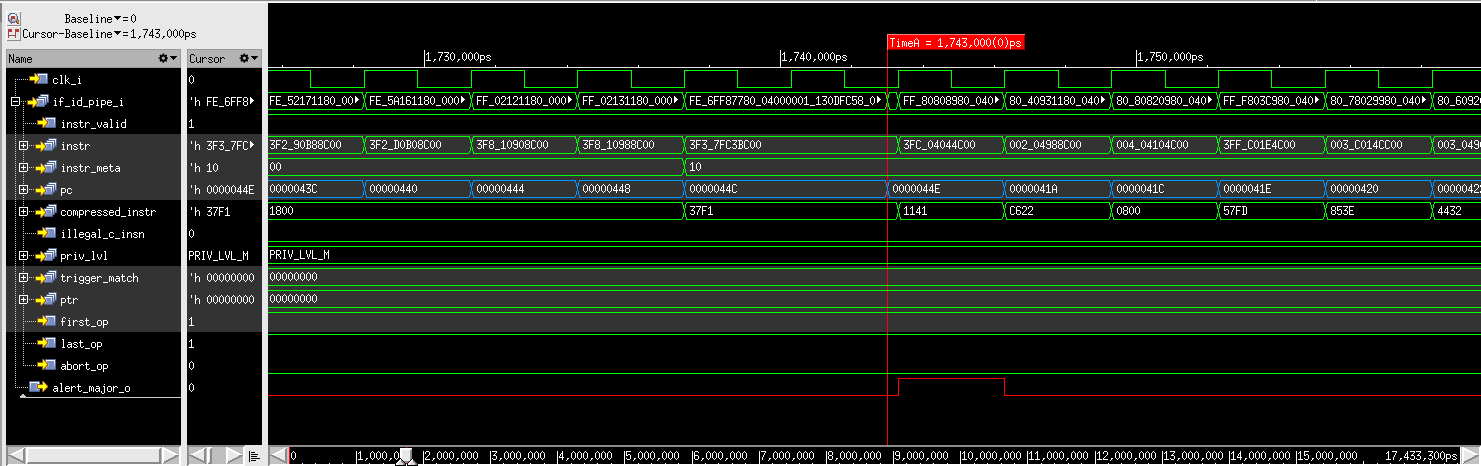
\includegraphics[width=\textwidth]{docs/images/instr_skip_glitch_injection_single_core.png}
    \caption{Waveforms from simulated instruction skip on CV32E40S.}
    \label{fig:instr_skip_single_wave}
\end{figure}

\subsubsection{Skipping out of while loop}

From the log file, we can see that the \textit{c.j} instruction is called 10 times. We skip the one logged at 1833ns. To skip this instruction the program counter needs to be skipped in the \textit{IF} stage, which is 3 cycles before the \textit{WB}. The \textit{c.j} is located at \textit{0x0000047a}. Forcing the program counter to the next address \textit{0x0000047c} for a duration of 3ns will simulate an instruction skip. This address is only 2 away because the \textit{j} is a 16-bit compressed instruction. 

Glitching out of the while loop was not successful. This is possibly due to other branch instructions from the loop that are also inside the pipeline. The attempted instruction skip is still detected and a major alert is raised. This can be seen in the simulation waveforms in \autoref{fig:instr_skip_loop_single_wave}. 

\begin{figure}[h!]
    \centering
    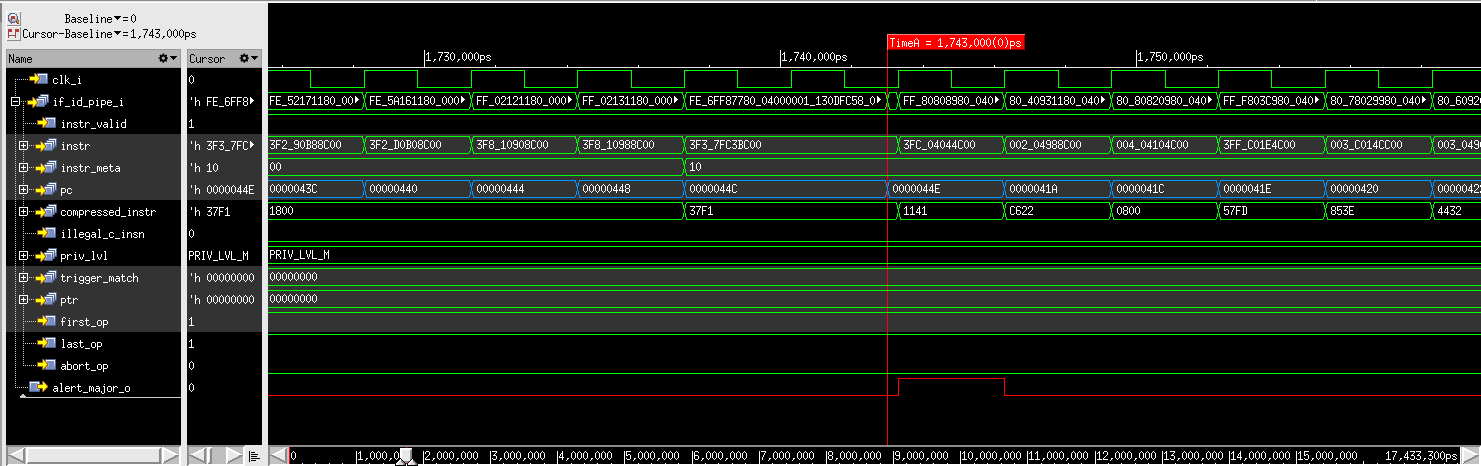
\includegraphics[width=\textwidth]{docs/images/instr_skip_glitch_injection_single_core.png}
    \caption{Waveforms from simulated instruction skip on CV32E40S.}
    \label{fig:instr_skip_loop_single_wave}
\end{figure}

\subsubsection{Skipping directly to end}

As mentioned earlier, an attacker can potentially glitch directly to the end of the program if they have some way of manipulating the code in the boot-loader. To simulate this, the program counter is forced to the address of the instruction after the while loop, \textit{0x00000482}. This force happens as soon as the main program is entered, which is at 1737ns.

This glitch attack was not successful. However, no major alert was raised by the core as can be seen in \autoref{fig:direct_skip_single_wave}. This glitch therefore bypassed the PCH feature. 

\begin{figure}[h!]
    \centering
    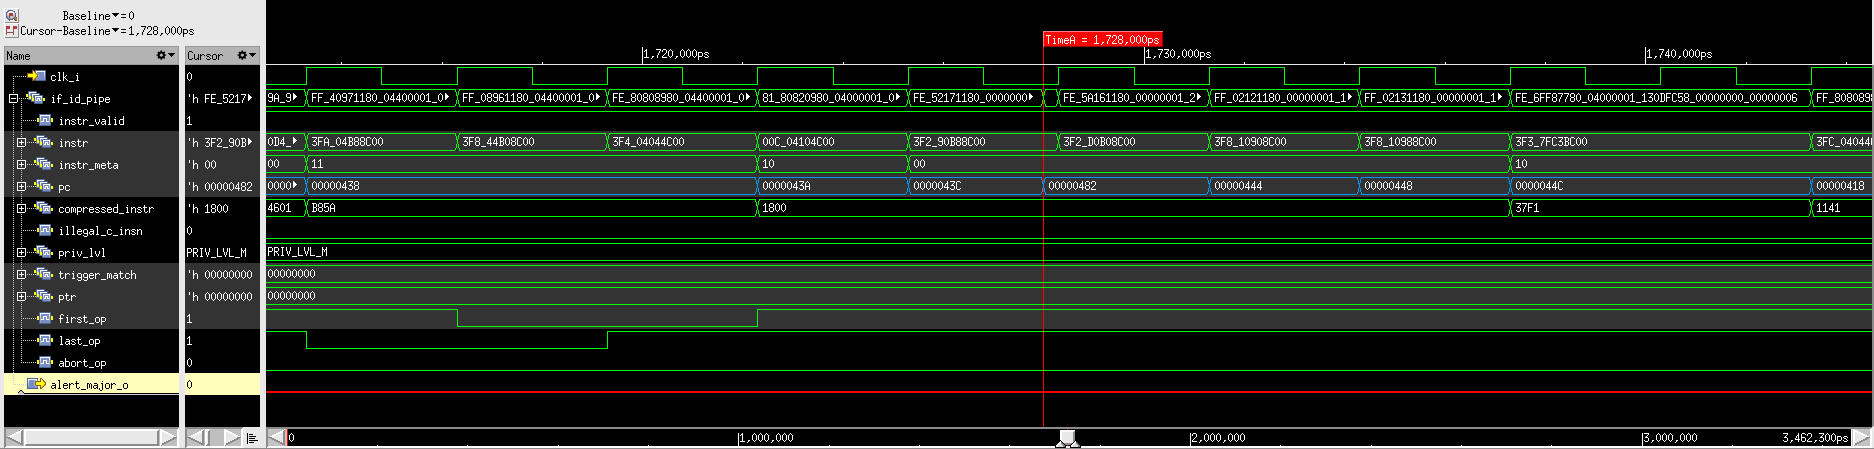
\includegraphics[width=\textwidth]{docs/images/direct_skip_single_core.png}
    \caption{Waveforms from simulated direct instruction skip on CV32E40S.}
    \label{fig:direct_skip_single_wave}
\end{figure}

\subsection{Dual-Core Lockstep}
\label{subsec:dual_instr_skip}

\subsubsection{Skipping function call}

The call to the \textit{c.jal} instruction occurs at 1707ns. The program counter is glitched to the address \textit{0x0000044e}. The 

\begin{figure}[h!]
    \centering
    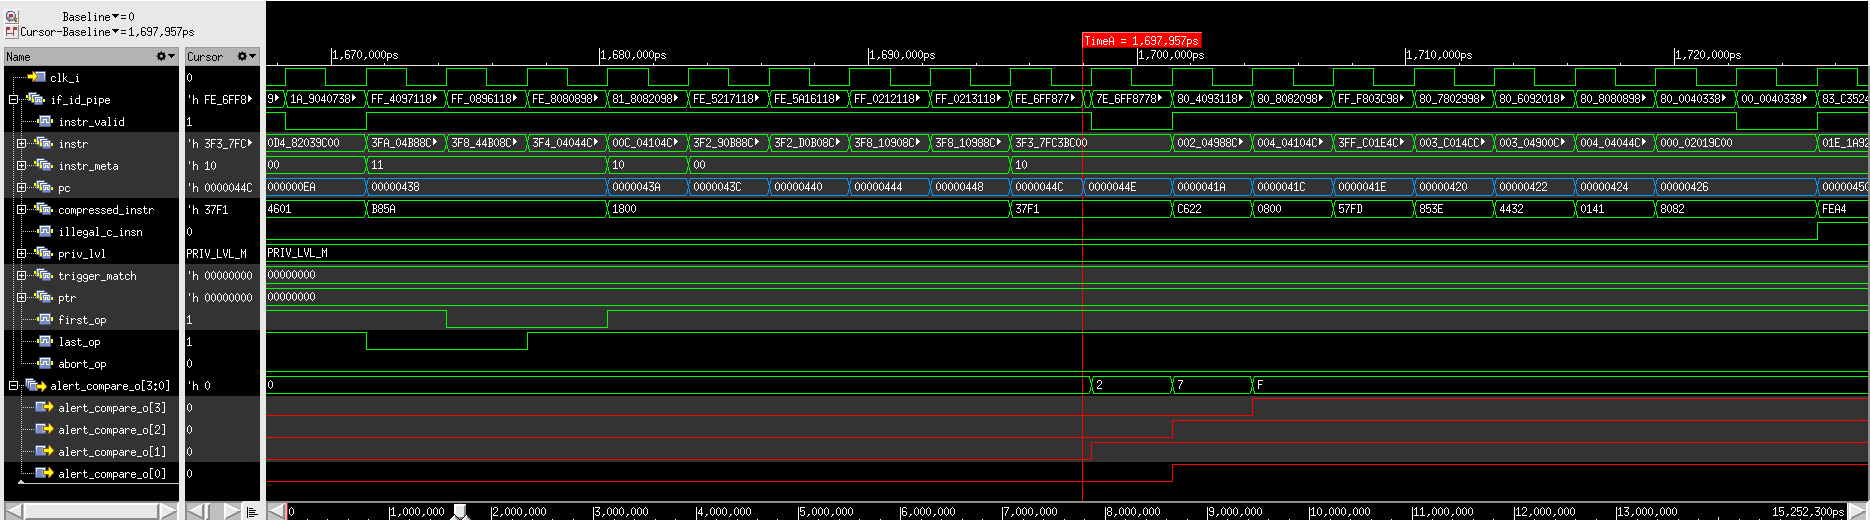
\includegraphics[width=\textwidth]{docs/images/instr_skip_dual_core.png}
    \caption{Waveforms from simulated instruction skip on Dual-Core Lockstep setup.}
    \label{fig:direct_skip_single_wave}
\end{figure}


\subsubsection{Skipping out of while loop}

The call to the \textit{c.j} instruction occurs first at 1782ns. The program counter is glitched to the address \textit{0x0000047c}.

\subsubsection{Skipping directly to end}

The call to the \textit{main} function occurs at 1689ns. The program counter is glitche dto the address \textit{0x00000482}.


\section{Coverage Test}
\label{sec:cov_test_result}



\textbf{Instruction to be glitched:}
\begin{lstlisting}
       30003.000 ns | 0000672c | memchr syscalls.c 379 - beq x14,x10,66b4 <memchr+0x3c>
\end{lstlisting}

In order to glitch the loop we need to make the program skip the instruction that happens at 29991.000 ns. This is a bne instruction that keeps us in the loop. Next instruction occurs at 29997 and we must therefore chang ethe program counter before this. 

Glitch 6734 to 673c

Count lagret i x8 
Verdien 10 lagret i x9

\section{Layout comparisons}

\subsection{Can this be implemented in read hardware?}
\begin{itemize}
    \item Compare performance 
    \item Compare area
    \item Compare Timing 
    \item Compare simulated power usage
    \item Compare glitch detection
\end{itemize}

\section{Why is this solution good/bad}

Synthesis results no pc hardening and dual core:

Area: 65214.732
Power: 1.44482mW

\chapter{Conclusion}
\label{chap6}

% Must be set after each chapter exept the first one in appendix.
\cleardoublepage

\appendix
\noappendicestocpagenum
\addappheadtotoc

\chapter{Appendix 1 - Code}
\label{app:appx1}

Any source code referenced in the project is shown in this appendix.

\section{hello-world simulation C-code}
\label{app:helloworldC}

\lstset{ 
   language=C,                   % choose the language of the code
   breaklines=true,                % sets automatic line breaking
   breakatwhitespace=false,        % sets if automatic breaks should only happen at whitespace
}
\begin{lstlisting}[caption={A sample C++ code}, label=lst:sample_code]
    /*
**
** Copyright 2020 OpenHW Group
**
** Licensed under the Solderpad Hardware Licence, Version 2.0 (the "License");
** you may not use this file except in compliance with the License.
** You may obtain a copy of the License at
**
**     https://solderpad.org/licenses/
**
** Unless required by applicable law or agreed to in writing, software
** distributed under the License is distributed on an "AS IS" BASIS,
** WITHOUT WARRANTIES OR CONDITIONS OF ANY KIND, either express or implied.
** See the License for the specific language governing permissions and
** limitations under the License.
**
*******************************************************************************
**
** Sanity test for the CV32E40S core.  Reads the MVENDORID, MISA, MARCHID and
**                                     MIMPID CSRs and prints some useful (?)
**                                     messages to stdout.  Will fail if these
**                                     CSRs do not match expected values.
**
*******************************************************************************
*/

#include <stdio.h>
#include <stdint.h>
#include <stdlib.h>

#define EXP_MISA 0x40901104

int main(int argc, char *argv[])
{

    volatile unsigned int misa_rval, mvendorid_rval, marchid_rval, mimpid_rval, mxl;
    volatile          int reserved, tentative, nonstd, user, super;

    mxl = 0; reserved = 0; tentative = 0; nonstd = 0; user = 0; super = 0;

    /* inline assembly: read mvendorid and misa */
    __asm__ volatile("csrr %0, 0xF11" : "=r"(mvendorid_rval));
    __asm__ volatile("csrr %0, 0x301" : "=r"(misa_rval));
    __asm__ volatile("csrr %0, 0xF12" : "=r"(marchid_rval));
    __asm__ volatile("csrr %0, 0xF13" : "=r"(mimpid_rval));

    /* Check MVENDORID CSR: 0x602 is the value assigned by JEDEC to the OpenHW Group */
    if (mvendorid_rval != 0x00000602) {
      printf("\tERROR: CSR MVENDORID reads as 0x%x - should be 0x00000602 for the OpenHW Group.\n\n", mvendorid_rval);
      return EXIT_FAILURE;
    }

    /* Check MISA CSR: if its zero, it might not be implemented at all */
    if (misa_rval != EXP_MISA) {
      printf("\tERROR: CSR MISA reads as 0x%x - should be 0x%x for this release of CV32E40S!\n\n", misa_rval, EXP_MISA);
      return EXIT_FAILURE;
    }

    /* Check MARCHID CSR: 0x15 is the value assigned by the RISC-V Foundation to CV32E40S */
    if (marchid_rval != 0x15) {
      printf("\tERROR: CSR MARCHID reads as 0x%x - should be 0x00000015 for CV32E40S.\n\n", marchid_rval);
      return EXIT_FAILURE;
    }

    /* Check MIMPID CSR: 0x0 is the value assigned by the OpenHW Group to the first release of CV32E40S */
    if (mimpid_rval != 0x00000000) {
      printf("\tERROR: CSR MIMPID reads as 0x%x - should be 0x00000000 for this release of CV32E40S.\n\n", mimpid_rval);
      return EXIT_FAILURE;
    }

    /* Print a banner to stdout and interpret MISA CSR */
    printf("\nHELLO WORLD!!!\n");
    printf("This is the OpenHW Group CV32E40S CORE-V processor core.\n");
    printf("CV32E40S is a RISC-V ISA compliant core with the following attributes:\n");
    printf("\tmvendorid = 0x%x\n", mvendorid_rval);
    printf("\tmarchid   = 0x%x\n", marchid_rval);
    printf("\tmimpid    = 0x%x\n", mimpid_rval);
    printf("\tmisa      = 0x%x\n", misa_rval);
    mxl = ((misa_rval & 0xC0000000) >> 30); // MXL == MISA[31:30]
    switch (mxl) {
      case 0:  printf("\tERROR: MXL cannot be zero!\n");
               return EXIT_FAILURE;
               break;
      case 1:  printf("\tXLEN is 32-bits\n");
               break;
      case 2:  printf("\tXLEN is 64-bits\n");
               break;
      case 3:  printf("\tXLEN is 128-bits\n");
               break;
      default: printf("\tERROR: mxl (%0d) not in 0..3, your code is broken!\n", mxl);
               return EXIT_FAILURE;
    }

    printf("\tSupported Instructions Extensions: ");
    if ((misa_rval >> 25) & 0x00000001) ++reserved;
    if ((misa_rval >> 24) & 0x00000001) ++reserved;
    if ((misa_rval >> 23) & 0x00000001) {
      printf("X");
      ++nonstd;
    }
    if ((misa_rval >> 22) & 0x00000001) ++reserved;
    if ((misa_rval >> 21) & 0x00000001) ++tentative;
    if ((misa_rval >> 20) & 0x00000001) ++user;
    if ((misa_rval >> 19) & 0x00000001) ++tentative;
    if ((misa_rval >> 18) & 0x00000001) ++super;
    if ((misa_rval >> 17) & 0x00000001) ++reserved;
    if ((misa_rval >> 16) & 0x00000001) printf("Q");
    if ((misa_rval >> 15) & 0x00000001) ++tentative;
    if ((misa_rval >> 14) & 0x00000001) ++reserved;
    if ((misa_rval >> 13) & 0x00000001) printf("N");
    if ((misa_rval >> 12) & 0x00000001) printf("M");
    if ((misa_rval >> 11) & 0x00000001) ++tentative;
    if ((misa_rval >> 10) & 0x00000001) ++reserved;
    if ((misa_rval >>  9) & 0x00000001) printf("J");
    if ((misa_rval >>  8) & 0x00000001) printf("I");
    if ((misa_rval >>  7) & 0x00000001) printf("H");
    if ((misa_rval >>  6) & 0x00000001) printf("G");
    if ((misa_rval >>  5) & 0x00000001) printf("F");
    if ((misa_rval >>  4) & 0x00000001) printf("E");
    if ((misa_rval >>  3) & 0x00000001) printf("D");
    if ((misa_rval >>  2) & 0x00000001) printf("C");
    if ((misa_rval >>  1) & 0x00000001) printf("B");
    if ((misa_rval      ) & 0x00000001) printf("A");
    printf("\n");
    if (super) {
      printf("\tThis machine supports SUPERVISOR mode.\n");
    }
    if (user) {
      printf("\tThis machine supports USER mode.\n");
    }
    if (nonstd) {
      printf("\tThis machine supports non-standard instructions.\n");
    }
    if (tentative) {
      printf("\tWARNING: %0d tentative instruction extensions are defined!\n", tentative);
    }
    if (reserved) {
      printf("\tERROR: %0d reserved instruction extensions are defined!\n\n", reserved);
      return EXIT_FAILURE;
    }
    else {
      printf("\n");
      return EXIT_SUCCESS;
    }
}

\end{lstlisting}

\subsubsection{Subsection}
Write something else here.

\lstset{language=matlab,breakautoindent, tabsize=1, breaklines, numbers=left, numberstyle=\tiny, numbersep=5pt, breakatwhitespace=true, frame=single, captionpos=tb, mathescape=true, basicstyle=\scriptsize}



\backmatter

%% PHD THESIS
\nocite{powerbook}

%% BOOKS
\nocite{tclbook}

%% ARTICLES
\nocite{digfil}

%% MISC
\nocite{convdef}

%% INPROCEEDINGS
\nocite{hwswMem}

%% TECHNICAL NOTES
\nocite{msp430f1611}

\newpage
\pagestyle{plain}
\addcontentsline{toc}{chapter}{Bibliography}
\bibliographystyle{alpha}
\bibliography{references/ref}

% Used with the make index package
\printindex
\end{document}
